\chapter{Discussion}
\label{chap:monocentric_discussion}

\begin{flushright}{\slshape    
It may be a small irony that  
just as\\
the phenomenon of polycentricity\\ is getting considerable attention,\\
The world is moving beyond it.} \\ \medskip
--- Peter Gordon \& Harry Richardson~\cite{Gordon:1996}
\end{flushright}


\bigskip


\section{Extending the model}
\label{sec:model}

Before concluding on the merits of the model and what we learn from it, and to
avoid mis-interpretations of its conclusions, it is necessary to state what the
model does not say and to present its limits.

\subsection{What the model does not say}
\label{sec:what_the_model_does_not_say}

\graffito{This discussion owes largely to questions raised during presentations
of this work.}

A first feature, hidden in the assumptions of the model, is that it does
not explain the concentration of activities in localised areas in the cities.
Rather, it takes the existence of centers as granted, and does not bother with
the behaviour of firms. Thereby, we do not pretend to explain the complexity of
urban dynamics in its entirety, but rather a single aspect of it. Of course,
this is a topic worthy of investigation, and should be studied seriously is one
wants to have a comprehensive understanding of the mechanisms that shape cities.

A second limitation lies in the description of congestion. In a worry of
simplificating the problem, we chose to adopt a macro-scale description of
traffic congestion, given by Eq.~\ref{eq:commuting_cost}. The sensitivity of the
road network to congestion is taken into account through the exponent $\mu$ and
the capacity $C$, which are assumed to be the same across the entire city. A
full specification of these parameters would need to understand how local
patterns of congestion lead to macroscropic behaviours at the city scale.  This
is, of course, a difficult entreprise:  local particularities of the layout may
have dramatic consequences on the fluidity of traffic, and congestions do
propagate through the network so that access to a given center can have an
effect on the travel to another center. 
Even without considering the difficult problem of modeling the behaviour of the
firms, and the way it is coupled to that of individuals, the model could be
improved in several ways. One first possible extension is to take the presence
of public transportation into account. Indeed, the model only considers
individual vehicles, prone to congestion, as a transportation mean.  However,
the largest cities in the world are all served by metro
systems~\cite{Roth:2012}, and the share of transports other than personal
vehicles can attain $42\%$\graffito{Number from the 2013 American Community
Survey} in cities like New-York. It is therefore far from being negligible, and
should somehow be taken into account in the model.
Still, cars remain the dominant mode of transportation in the
US, as shown of Fig.~\ref{fig:transportation_mode}. The use of alternative modes
of transportation is only notable in New-York, which is already a polycentric
city.\\

\begin{figure}[!h]
    \centering
    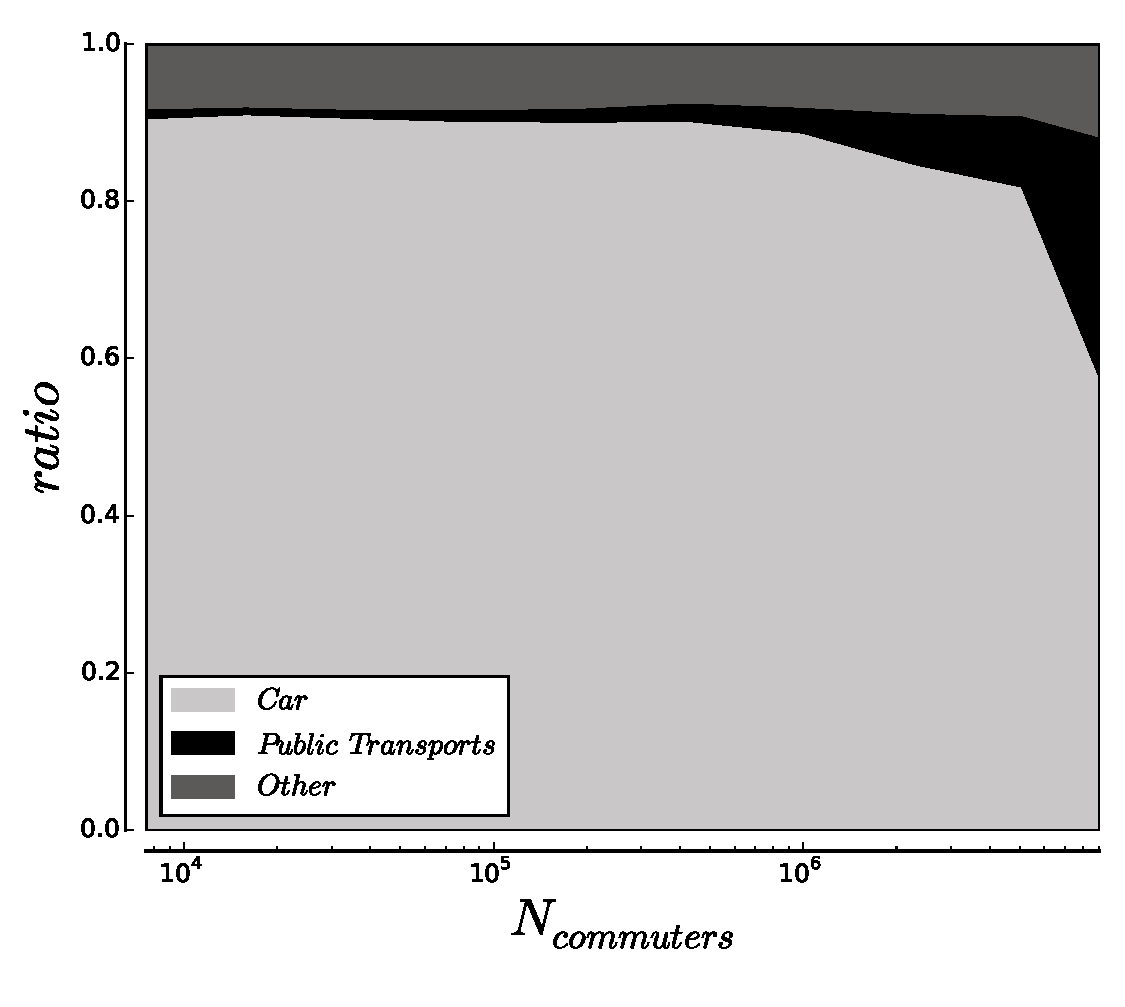
\includegraphics[width=0.8\textwidth]{gfx/chapter-monocentric/transportation_modes.pdf}
    \caption{Importance of different transportation modes in US Metropolitan
    Statistical Areas, as a function of the number of commuter. Although the
proportion of individuals using public transportation or other modes (walking,
cycling, working at home) increases with population size, cars stay the dominant
mode of transportation everywhere. Data from the 2013 American Community
Survey.\label{fig:transportation_mode}}
\end{figure}


Another limitation of the model is the assumptions that all individuals are
identical, in the sense that they can all pretend to the same wage. Adding an
income structure into the model could allow us to explore the spatial patterns
of segregation, and see whether they can be understood from basic economical
choices alone. In fact, while perusing the economics literature on the
topic~\cite{Glaeser:2008, Brueckner:1999}, we realised that there was very little
empirical knowledge on segregation that could be used to test a model. This led
us to the study that we present in part~\ref{part:stratification} of this
thesis.\\

\medskip

\section{Shadows in the empirical picture}
\label{sec:empirical}

\subsection{Measuring the number of centers}
\label{sub:measuring_the_number_of_centers}

There is also some work left to be done on the empirical side. Although
non-parametric methods are an improvement over the previous parametric methods,
we are yet to understand what the meaning of the obtained centers is. In
particular, a problem that remains with non-parametric methods is that, no
matter the distribution of employment, population, etc. into the areal units,
the method will output a number. In the extreme case of a city where employment
would be uniformly distributed in space, the LouBar method would tell us that
the number of centers is equal to the number of areal units. Yet, can we really
talk about centers in this case? Most would object, and ironically invoke common
sense. The difficulty resides in that we do not know what we mean exactly when
we talk about centers: do they reflect an objective reality, or are they a mere
artifact of the way our brains process information? In the latter case,
parametric methods will do just fine, while the former case means we need to
understand what we talk about when we talk about centers.  

A further shortcoming of current methods to determine the number of subcenters
is that they do not consider the spatial arrangement of the areal units
involved. This can be problematic when the method identifies areal units that
are contiguous as center. On Fig.~\ref{fig:hotspots_boston} we show an example
of such a situation. We use the LouBar method~\cite{Louail:2014} to extract the
employment hotspots in the Metropolitan Statistical Area of Boston using data
from the 2000 Census. As one can see, several of the hotspots thus identified
are indeed contiguous. Should we still count them as separate hotspots? Or
should we consider that all contiguous hotspots are part of a larger hotspots
that encompasses them all? 

\begin{figure}[!h]
    \centering
    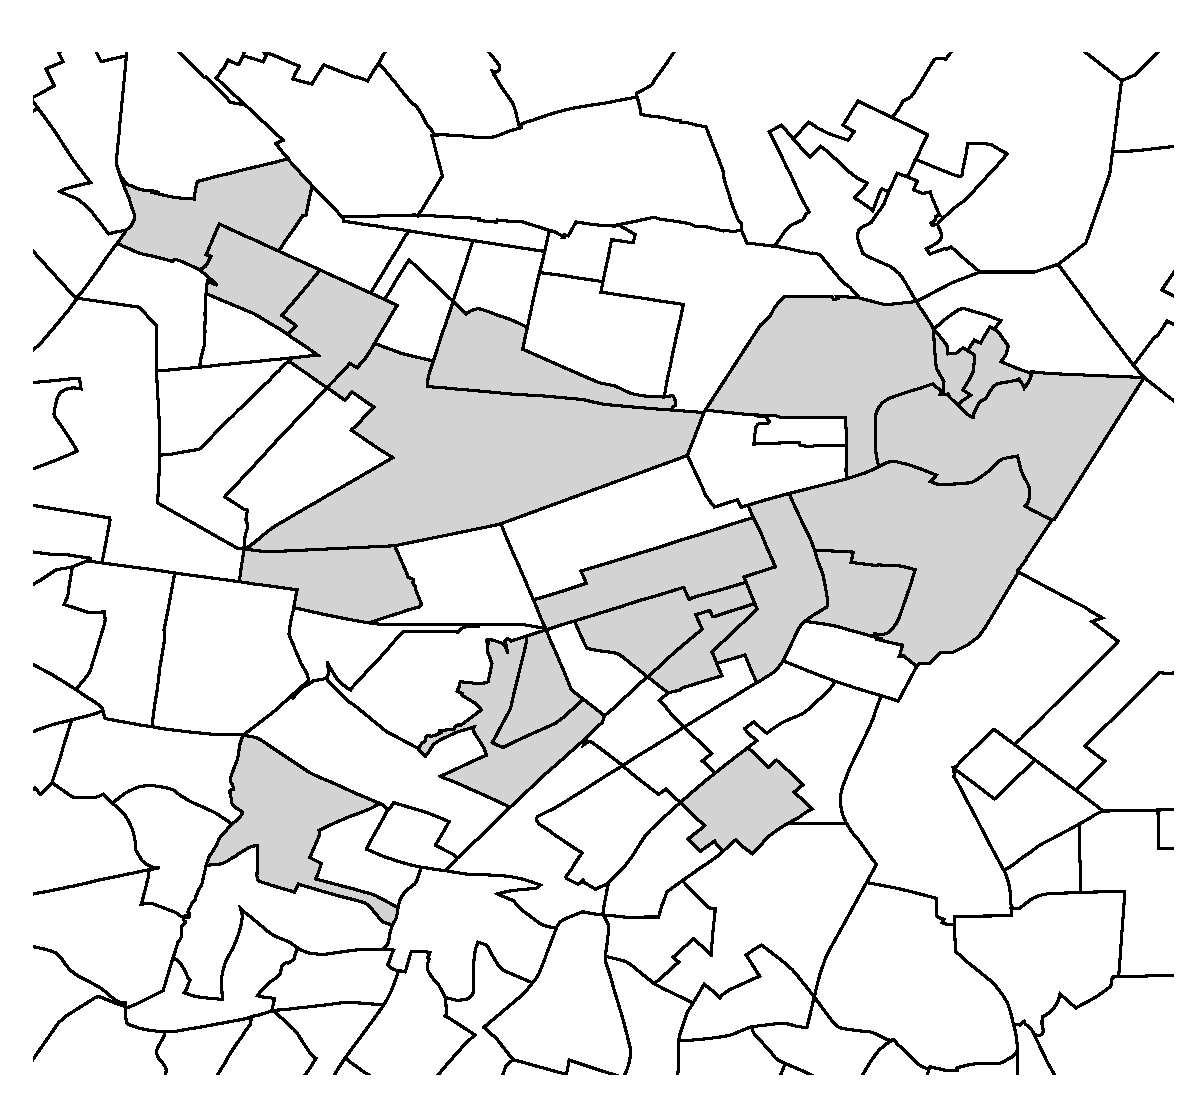
\includegraphics[width=0.75\textwidth]{gfx/chapter-monocentric/hotspots_boston.pdf}
    \caption{The census tracts of downtown Boston, MA in the US. In light grey,
    the census tracts that are identified as employment hotspots by the LouBar
method. Although the method designates all light grey tracts as different hotspots,
many of them are contiguous. We can wonder whether such contiguous
hotspots are, in fact, part of a larger hotspot that would include all of them.
This plot was generated with python, using the 2000 Census tract-to-tract
commuting flows and the 2000 Census tracts geometry.\label{fig:hotspots_boston}}
\end{figure}

This problem is in fact very general, and pertains to the field of spatial
analysis (including spatial statistics). Finding centers indeed amounts to
finding the proper way to describe a density profile at a meso-scale level and
to devising proper methods to detect the salient feature of this spatial
pattern. The tools provided by spatial analysis are however not yet suited to
provide such a description. This would however have huge potential applications.
With hindsight, such tools would also help to describe the spatial patterns of
segregation that we study in part \ref{part:stratification} of this
manuscript.

The results of the methods provided in the introduction should not be thrown
away altogether, though. The number of centers they provide probably does not
reflect the `real' number of centers (if there is such a thing) in a particular
city. But, assuming that different cities exhibit similar structures, they
should still provide values that are coherent across different urban areas, and
are thus useful for \emph{comparison} purposes.\\


\subsection{Beyond polycentricity}
\label{sec:beyond_polycentricity}


\subsubsection{The dispersed city}
\label{sub:the_dispersed_city}

Progressively, the concept of the monocentric city got replaced with the more
elaborate polycentric hypothesis. Is that the end of the story? As suggested in
the quote opening this chapter, reality is not that straightforward. Gordon and
Richardson, in a provocative article~\cite{Gordon:1996}, argue that, rather than
polycentric, cities are dispersed. Indeed, studying the employment density in
Los Angeles, they found that the centers they defined based on density only contained $17\%$ of
the total employment. Hardly a polycentric situation! 
Of course, we can wonder whether Gordon and Richardson's results are an artefact
of the choice of their case study --Los Angeles, famous for its sprawl-- or the particular method they
used to compute the number of centers. For this reason, we plot on
Fig.~\ref{fig:concentration_loubar} the ratio of the total number of individuals that is contained
in the centers defined by the LouBar method. The results are striking: only a
few, small metropolitan area reach the mark where $50\%$ of individuals
(employees or residents belong) to a designed center. Worse, cities seem to be
on average more dispersed as they are bigger.\\

\begin{figure}
    \centering
    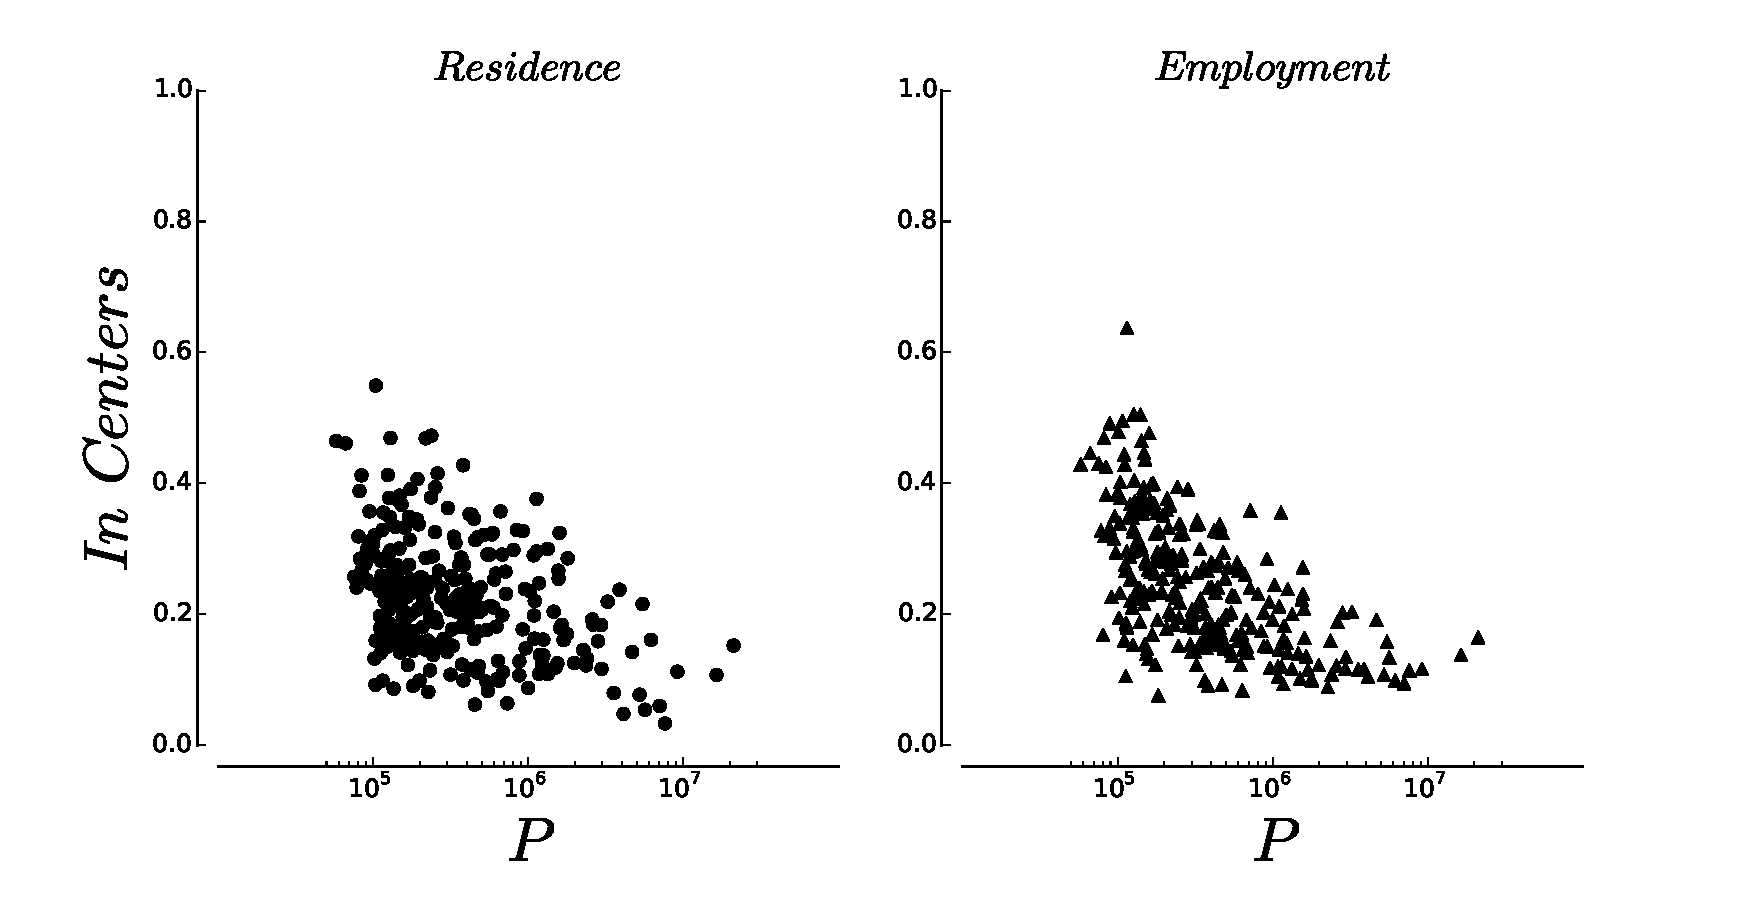
\includegraphics[width=1\textwidth]{gfx/chapter-monocentric/concentration_loubar.pdf}
    \caption{{\bf Concentration in subcenters.} (Left) Ratio of the total
    residential population in US MSAs that lives in the centers identified by the LouBar
method. (Right) Ratio of the total number of employees in US MSAs that works in the centers
identified by the LouBar method. Overall, cities are very dispersed, with only a
few cities having more than $50\%$ of their workforce or residential population
living in centers, confirming the results of Gordon and
Richardson~\cite{Gordon:1996}. Data were obtained for the 2000 US Census, the
figure was prepared using Python.\label{fig:concentation_loubar}}
\end{figure}

The lesson that should be learned from the article by Gordon and Richardson is
that the notion of polycentricity is \emph{also an hypothesis} on the spatial
structure of densities. While it is arguably more involved than the monocentric
hypothesis, it does indeed consists in imposing some structure onto the raw
data. The process itself of counting centers implies that these centers exist,
that there is an element of reality attached to what we call centers. A quick
look on the 3D plot shown on Fig.~\ref{density_3d} should convince the reader
that the world is not as simple as the way we picture it. While employment
densities indeed exhibit strong peaks that are easily distinguishible (although
that is arguable for Houston), the same cannot be said for population densities.
The point, I argue, is not that the monocentric or the polycentric model are
wrong alltogether. The problem lying more in the lack of appropriate tools to
describe a density spatial profile, in the fact that there is no `one size fits
all' method of analysis. Indeed, the exploratory tools presented above, as well
as the ones presented in the following section, try to fit a certain model of
the city to the actual data, be it monocentric or polycentric.\\

\subsubsection{Quantifying Urban form}
\label{sub:urban_form}

\cite{Tsai:2005} is a classic on Urban Form, along with~\cite{LeNechet:2015} and
\cite{Schwarz:2010}.
Have a look at what~\cite{Berroir:2008} do!
\cite{Bertaud:2001} is very interesting on urban form in general, and proposes
an index, the eccentricity, to measure the distance of the center of gravity to
the geographical CBD.
\cite{LeNechet:2010} introduces the acentrism index (also explained
in~\cite{LeNechet:2015}.\\
\cite{Pereira:2013} proposes an Urban Centrality Index that varies continuously
between a monocentric configuration and an extreme decentralized situation.

\section{Summary}
\label{sec:summary}

In this part, we have presented an historical overview of the monocentric
hypothesis for the structure of cities, and how the view has progressively
shifted towards the picture of a more distributed, polycentric organisation.
Starting with indirect evidence for a polycentric picture, several methods were
then naturally proposed to directly measure the number of centers, from the
first parametric methods to the more recent non-parametric methods. Observing
evidence for an increased polycentricity with population size, we then wondered
what were the possible explanations for this phenomenon. We proposed an
out-of-equilibrium model of city growth that predicts the necessary emergence of
secondary centers as populations grows, and a sublinear increase of the number
of subcenters with population---both verified on empirical data, across
different countries, for several city definitions.

In the next part, we will continue our journey with another, seemingly unrelated
topic: scaling relationships. We will start with an historical perspective on
 scaling, showing that scaling relationships are older than most people believe,
 and we will provide a non-exhaustive review of the empirical results. We will
 then be ready to show how, using the model exposed in this chapter, we can
 understand the scaling relationships related to mobility in cities. We will
 then conclude on a reflection of what scaling relationships can and do tell us about cities,
 and highlight their shortcomings.
